\section{Durchführung}

Das verwendete Viskosimeter ist in Abbildung \ref{fig:Aufbau} dargestellt. 

\begin{figure}
\center
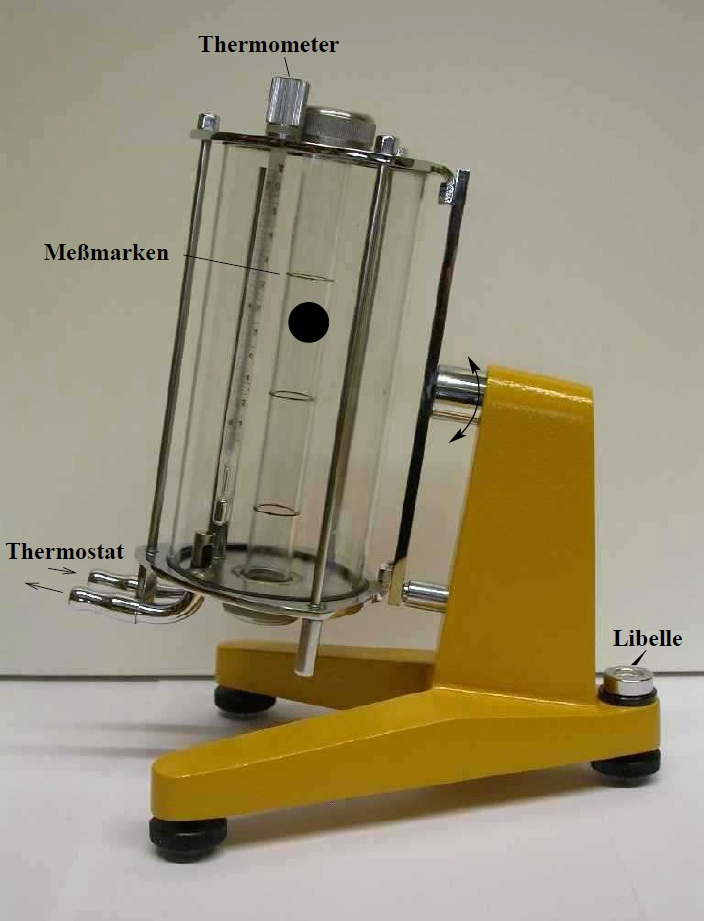
\includegraphics[scale=0.3]{content/Aufbau.jpg}
\caption{Höppler Viskosimeter}
\label{fig:Aufbau}
\end{figure}

Drei an dem inneren Rohr befindliche Messmarken makieren eine Strecke 
von \SI{10}{\centi\meter}. Umgeben wird das Rohr von Wasser, dessen 
Temperatur durch ein angeschlossenes Thermostat samt Pumpe geregelt wird. 
An einem Thermometer kann die momentane Temperatur abgelesen werden. 
Durch Abschrauben des Deckels kann das Glasrohr im Inneren mit dem Fluid und 
der Kugel befüllt werden. Die gesamte Zylinderstruktur lässt sich um 
180° rotieren. Eine Libelle zeigt an, ob sich der Aufbau in Waage
befindet. Für das Experiment stehen zwei Glaskugeln mit unterschiedlichen
Radien zur Verfügung. 

Zunächst werden die Radien der beiden Glaskugeln und das Gewicht mit einer 
Waage bestimmt. Daraus lässt sich jeweils die Dichte bestimmen. 
Danach wird das Viskosimeter in Waage gebracht und anschließend mit destilliertem Wasser 
befüllt. Entstandene Luftblässchen werden mit einem Glasstab entfernt und 
danach die kleinere der beiden Kugeln in die Flüssigkeit eingetaucht. Das 
Viskosimeter wird verschlossen und mit Stopuhr gemessen, wielange die Kugel benötigt, 
um die \SI{10}{\centi\meter} Flüssigkeit bei Raumtemperatur zu durchlaufen. 
Der Vorgang wird durch kippen des Glaszylinders insgesamt 10 Mal wiederholt, 
bevor auch die zweite Kugel auf die selbe Art verwendet wird. Es entstehen 
folglich für jede Kugel 10 Messwerte. Außerdem wird die Temperatur des Wassers
notiert. 

Da man nun auch die Temperaturabhängigkeit messen will, wird das Thermostat
angeschaltet. Das Wasserbad wird bis zu 70°C aufgeheizt. 
Auf diese Weise werden für die große Kugel Fallzeiten bei 10 
Temperaturen von 21.5°C bis 70°C ermittelt.
Jede Fallzeit wird dabei zwei Mal gemessen. 


\label{sec:Durchführung}
